\documentclass{article}

\usepackage{RepSty}
\usepackage{SPINDefs}
\usepackage{hyperref}

\usepackage{setspace}
\usepackage{multirow}
\usepackage{threeparttable}
\usepackage{paralist}

\usepackage[caption=false]{subfig}

\newcommand{\bld}{\boldsymbol}
\newcommand{\Wx}{\Omega_x}
\newcommand{\Wy}{\Omega_y}
\newcommand{\Dt}{\Delta t}

\begin{document}
	\singlespacing
	\begin{titlepage}

\begin{center}
{МИНИСТЕРСТВО ОБРАЗОВАНИЯ И НАУКИ РОССИЙСКОЙ ФЕДЕРАЦИИ}\\[3pt]
\textsc{\small{Федеральное государственное автономное образовательное учреждение высшего образования}}\\

\textbf{\enquote{Национальный исследовательский ядерный университет\\
{``МИФИ''}}}\\
\textbf{(НИЯУ МИФИ)}\\[2cm]




\textsc{\textbf{Отчет о научно-исследовательской деятельности\\		
		аспиранта и подготовке научно-квалификационной\\	
		работы (диссертации) на соискание ученой степени\\		
		кандидата наук за торое полугодие 3 курса}}\\[2cm]

% Title
\enquote{Изучение магнитооптических структур в системах Замороженного и Квази-замороженного спина}\\[2cm]


\end{center}


\begin{flushleft}
% Author and supervisor
\begin{tabular}{ll}
Аспирант 						& А.Е. Аксентьев \\
Направление                     & 03.06.01 Физика и астрономия \\					
Научная специальность		   	& 01.04.20 Физика пучков заряженных частиц\\
								& \-\hspace{1.8cm} и ускорительная техника \\[1cm]
Научный руководитель 			& \\
Должность, степень, звание 		& С.М. Полозов, к.ф.-м.н, доц. \\[1cm]
Дата защиты:					& \\
Результат защиты:				& \\
\end{tabular}

\end{flushleft}

\vfill


\begin{center}
Москва \the\year{}
\end{center}



\end{titlepage}
	
	\tableofcontents 
	\pagebreak
	
	\onehalfspacing
	
	\section*{Физическая мотивация}
	 Вся наблюдаемая вселенная состоит преимущественно из материи; антиматерия может быть получена в ускорителях заряженных частиц, но в пренебрежимо малых количествах. На сегодняшний день считается, что вскоре после Большого Взрыва материя была образована из энергии в парах частица-античастица, после чего последовала стадия аннигиляции; однако, по какой-то причине, эта фаза закончилась превалированием материи над антиматерией (по крайней мере в наблюдаемой вселенной) --- процесс называемый \emph{бариогенезом.}
	
	В 1967 году, академик АН СССР Андрей Сахаров определил условия, требуемые для бариогенеза (независимо от механизма его действия). Одно из \emph{условий Сахарова} --- существование процессов, нарушающих C- и CP-симметрии. Известны источники нарушения этих симметрий, однако их не достаточно для объяснения барионной асимметрии вселенной; поиск продолжается.
	
	Интерес поиска Электрического Дипольного Момента (ЭДМ) элементарных частиц состоит в том, что, если они существуют, то они нарушают P- и T-симметрии. Таким образом, обнаружение ненулевых ЭДМ элементарных частиц может привести нас к физике за границами Стандартной Модели; такие теории как SUSY (суперсимметрия) указывают на наличие ЭДМ гораздо большей величины (на уровне $10^{-29} - 10^{-24}$ e$\cdot$cm), чем предсказывает Стандартная Модель.
		
	\section{Состояние изучаемой проблемы}
	Поиск ЭДМ в невырожденных системах был инициирован Эдвардом Пёрселлом и Норманом Рэмзи более 50 лет назад, для нейтрона. С тех пор было проведено множество всё более чувствительных экспериментов на нейтронах, атомах, и молекулах, и тем не менее, ЭДМ пока ещё не был обнаружен. На данный момент, верхний предел ЭДМ нейтрона оценивается на уровне $<3\cdot 10^{-26}$ e$\cdot$cm, протона --- $<8\cdot 10^{-25}$ e$\cdot$cm.~\cite{Pretz_presentation}
	
	В 2008 году коллаборацией в Брукхейвенской Национальной Лаборатории (BNL, США) был предложен эксперимент по измерению ЭДМ дейтрона, основанный на использовании эффекта замороженного спина в магнитном накопительном кольце.~\cite{BNL} 
	
	В 2015 году, коллаборацией Storage Ring EDM Collaboration, был предложен эксперимент по поиску протонного ЭДМ в полностью электрическом накопительном кольце.~\cite{Proton_EDM}
	
	На данный момент, коллаборацией JEDI (Исследовательский центр ``Юлих,'' Германия) ведётся разработка структуры накопительного кольца для проведения предварительного эксперимента по измерению дейтронного ЭДМ на синхротроне COSY.
	
	\subsection{Предложение BNL}\label{sec:BNL_Proposal}
	Движение спина частицы в электромагнитном поле описывается уравнением Томаса-Баргманна-Мишеля-Телегди:
	\begin{equation*}
	\begin{cases}
	\sfrac{\td\bld S}{\td t} &=\bld S \times\bld \Omega,\\
	\bld \Omega &= -\frac em \bkt*{G\bld B + \bkt{\frac 1 {\gamma^2 - 1} - G}\bld \beta \times\bld E + \frac\eta2 \bkt{\bld E +\bld\beta\times\bld B}}.
	\end{cases}
	\end{equation*}
	Здесь, $G = (g-2)/2$ --- аномальный магнитный момент; для дейтрона $G = -0.142$. Подобрав энергию частицы, можно ``заморозить'' направление её спина относительно импульса; это называется условием \emph{замороженного спина}.
	
	В концепции эксперимента, предложенного BNL~\cite{BNL}, продольно поляризованный пучок инжектируется в накопительное кольцо. При соблюдении условия замороженного спина, вектор поляризации пучка в горизонтальной плоскости сонаправлен с вектором импульса в любой момент времени. Засчёт присутствия радиальной компоненты электрического поля, при условии отличного от нуля ЭДМ, спин будет медленно поворачиваться в вертикальной плоскости. Измеряя вертикальную компоненту поляризации по истечении значительного промежутка времени, можно вычислить $\eta$. 
	
	Такая методология ограничена, в первую очередь, конечным временем когеренции спина (SCT). Декогеренция спина обусловлена различием длин орбит частиц в пучке, что в свою очередь есть результат конечности фазового объема пучка. Раскладывая выражение для спин-тюна частицы в электро-мангитном поле вокруг референсного значения получим:~\cite{SenichevRuPAC2016}
	\begin{equation*}
		\begin{cases}
		\Delta\nu_s^E &= G_6\Delta\gamma + O(\Delta\gamma),\\
		\Delta\nu_s^B &= G\Delta\gamma,\\
		\Delta\gamma(t) &= \Delta\gamma_m\cos(\Omega_s t) + f(\alpha_1, \eta, \gamma)\Delta\gamma_m^2 + g\bkt{\eta, \beta, \frac{\Delta L}{L}}\gamma^2.
		\end{cases}
	\end{equation*}
	Здесь: $G_6$ есть некоторая функция $(G, \gamma_0)$, $\Delta\gamma_m, \Omega_s$ --- амплитуда и частота синхроторонных колебаний, $\alpha_1$ коэффициент сжатия орбиты , $\eta$ --- слип-фактор, $\Delta L/L$ --- удлинение орбиты засчёт бетатронных колебаний.
	
	Первый член $\Delta\gamma(t)$ усредняется в ноль засчёт синхротронных колебаний; используя секступольные магниты можно уменьшить декогеренцию, связанную с удлинением орбиты.
	
	
	\subsection{Структуры FS и QFS колец}
	Полезный ЭДМ сигнал максимален при соблюдении условия замороженного спина; однако, это условие требует чтобы у частицы было конкретное ``магическое'' значение энергии. Таким образом, это условие не может быть выполнено для всех частиц в пучке. На практике, это условие выполняется только для референсной частицы. Также, в замороженном (FS) кольце требуется использование комбинированных E+B элементов в арках, что усложняет конструкцию ускорителя. По этим причинам, была предложена концепция кольца с квази-замороженным спином (QFS).
	
	В QFS кольце не требуется непрерывное выполнение FS условия; спин частицы возвращается в ``замороженное'' положение специальной оптикой через каждые $n$ оборотов. При прецессии спина в горизонтальной плоскости с амплитудой $\Phi_s$, рост ЭДМ-сигнала спадает пропорционально $J_0(\Phi_s) \approx 1 - \bkt{\frac{\Phi_s}{2}}^2$. Таким образом, для дейтронного кольца с $G = -0.142$, при амплитуде прецессии $\Phi_s = \pi\cdot\sfrac{\gamma G}{2n}$, деградация сигнала не превышает нескольких процентов. Также, эта структура может быть выполнена в двух вариантах: 
	\begin{inparaenum}[1)]
		\item с искривлёнными прямыми секциями с цилиндрическими электростатическими дефлекторами,
		\item с прямыми комбинированными E+B дефлекторами в прямых секциях.
	\end{inparaenum}~\cite{SenichevICAP15}

	\begin{figure}
		\centering
		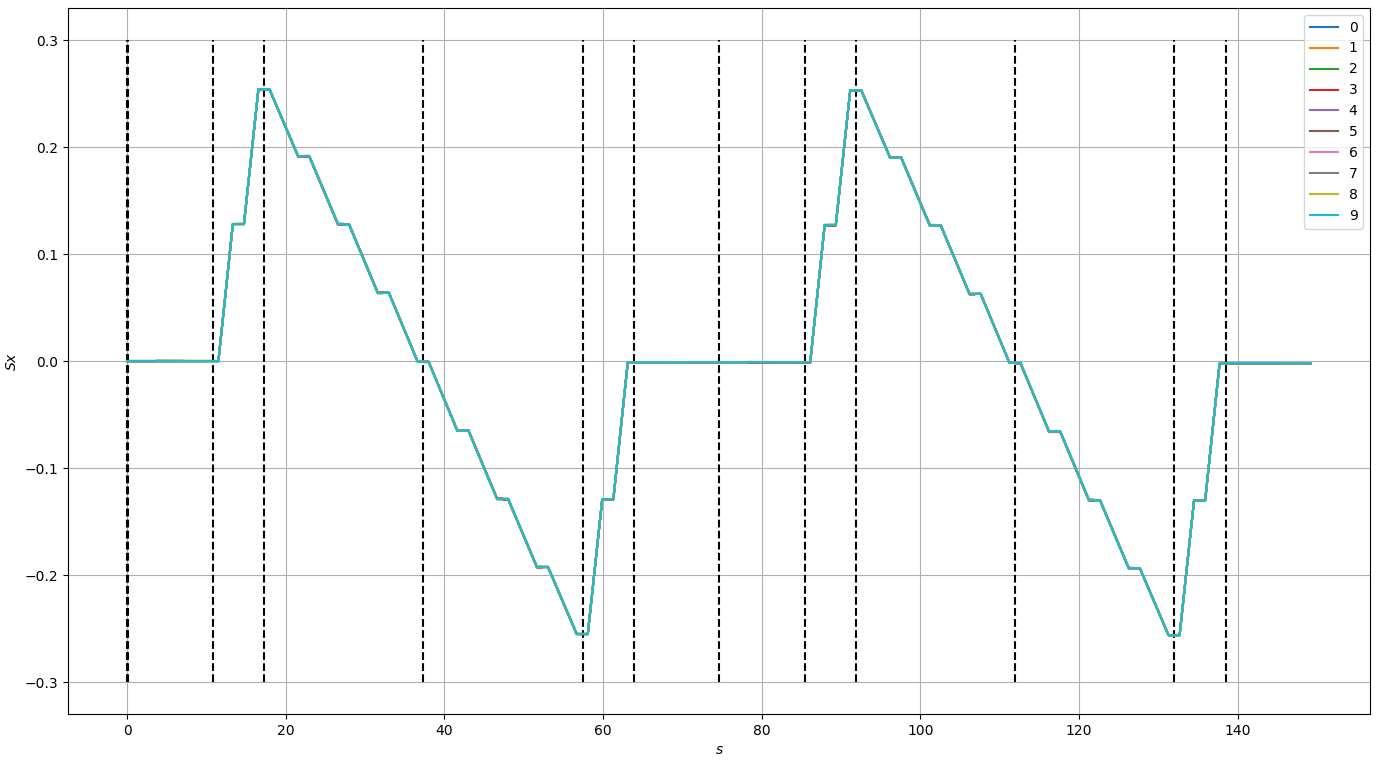
\includegraphics[scale=.5]{edm_img/EB_QFS_Sx_vs_s_1turn}
		\caption{Эволюция радиальной компоненты спина частиц в QFS структуре на длине одного оборота. Вертикальные пунктирные линии обозначают границы секций ускорителя.}
	\end{figure}
	
	\section{Цели и задачи работы}
	Целью данной работы является сравнение структур FS и QFS для определения которая из них больше подходит для проведения эксперимента по поиску ЭДМ дейтрона с точностью $10^{-29}$ e$\cdot$cm.
	
	Для этого предложена следующая программа:
	\begin{enumerate}
		\item Изучение эффекта неточности установки E+B элементов (сохраняется сила Лоренца) в FS-структуре на спин-динамику пучка;
		\item То же самое для квадрупольных магнитов (сила Лоренца не сохраняется);
		\item Изучение зависимости декогеренции спина от начального распределения пучка по поперечным координатам и энергии;
		\item Изучение оптимальной расстановки секступольных магнитов с целью подавления декогеренции и хроматичности;
		\item Моделирование калибровки магнитного поля в ускорителе по параметру $\gamma_{eff}$ в горизонтальной плоскости для процедуры CW/CCW.
	\end{enumerate}

	\section{Текущий статус}
	\subsection{Трекинговый код}
	Для проведения анализа был написан код на языке Python. В данном коде используется поэлементное интегрирование системы уравнений описанных в~\cite[стр. 39]{Ivanov_thesis}. Наклон элементов имплементирован в двух вариациях:
	\begin{inparaenum}[1)]
		\item путём вычисления ротационной матрицы (метод работает для всех элементов, но он медленный);
		\item специализированное преобразование полей в E+B элементах и квадруполях.
	\end{inparaenum}
	Во втором методе моделирования наклона элементов, при наклоне E+B сохраняется вертикальная копонента магнитного поля; также добавляется копенсирующее вертикальное электрическое поле, для сохранения силы Лоренца (соответственно, орбитального движения), действующей на частицу. При наклоне квадруполя, добавляется дипольная компонента поля, но сила Лоренца (соответственно орбитальное движение частицы) при этом нарушается.
	
	\paragraph{Моделирование декогеренции пучка}
	Для изучения декогеренции пучка в вертикальной и горизонтальной плоскостях был промоделирован следующий эксперимент:
	\begin{itemize}
		\item Три пучка по 1,000 частиц: $X \sim N(0, 10^{-3}),\, Y \sim N(0, 10^{-3}), \, \Delta K \sim N(0, 10^{-4})$.
		\item Все частицы инжектированы со спином $\bld S(0) = (0, 0, 1)$.
		\item Трекинг на 100 оборотов в FS структуре со случайно-наклонёнными E+B элементами; угол наклона выбран из $N(0, 10^{-4})$;
		\item Собиралась статистика: $\Wx = S_y(100)/\Dt(100)$ и $\Wy = S_x(100)/\Dt(100)$.
	\end{itemize}

	Результаты моделирования представлены на рисунке~\ref{fig:decoherence_test}. Поскольку средняя величина радиальной компоненты магнитного поля пропорциональна среднему углу наклона E+B элементов, из уравнения Т-БМТ ожидается линейная зависимость роста радиальной компоненты спин-тюна $\Wx$ для референсной частицы. В FS структуре, $\Wy$  референсной частицы должно быть в области нуля.

	\begin{figure}[htb]
		\centering
		\subfloat[Линейный характер зависимости соответствует уравнению Т-БМТ.]{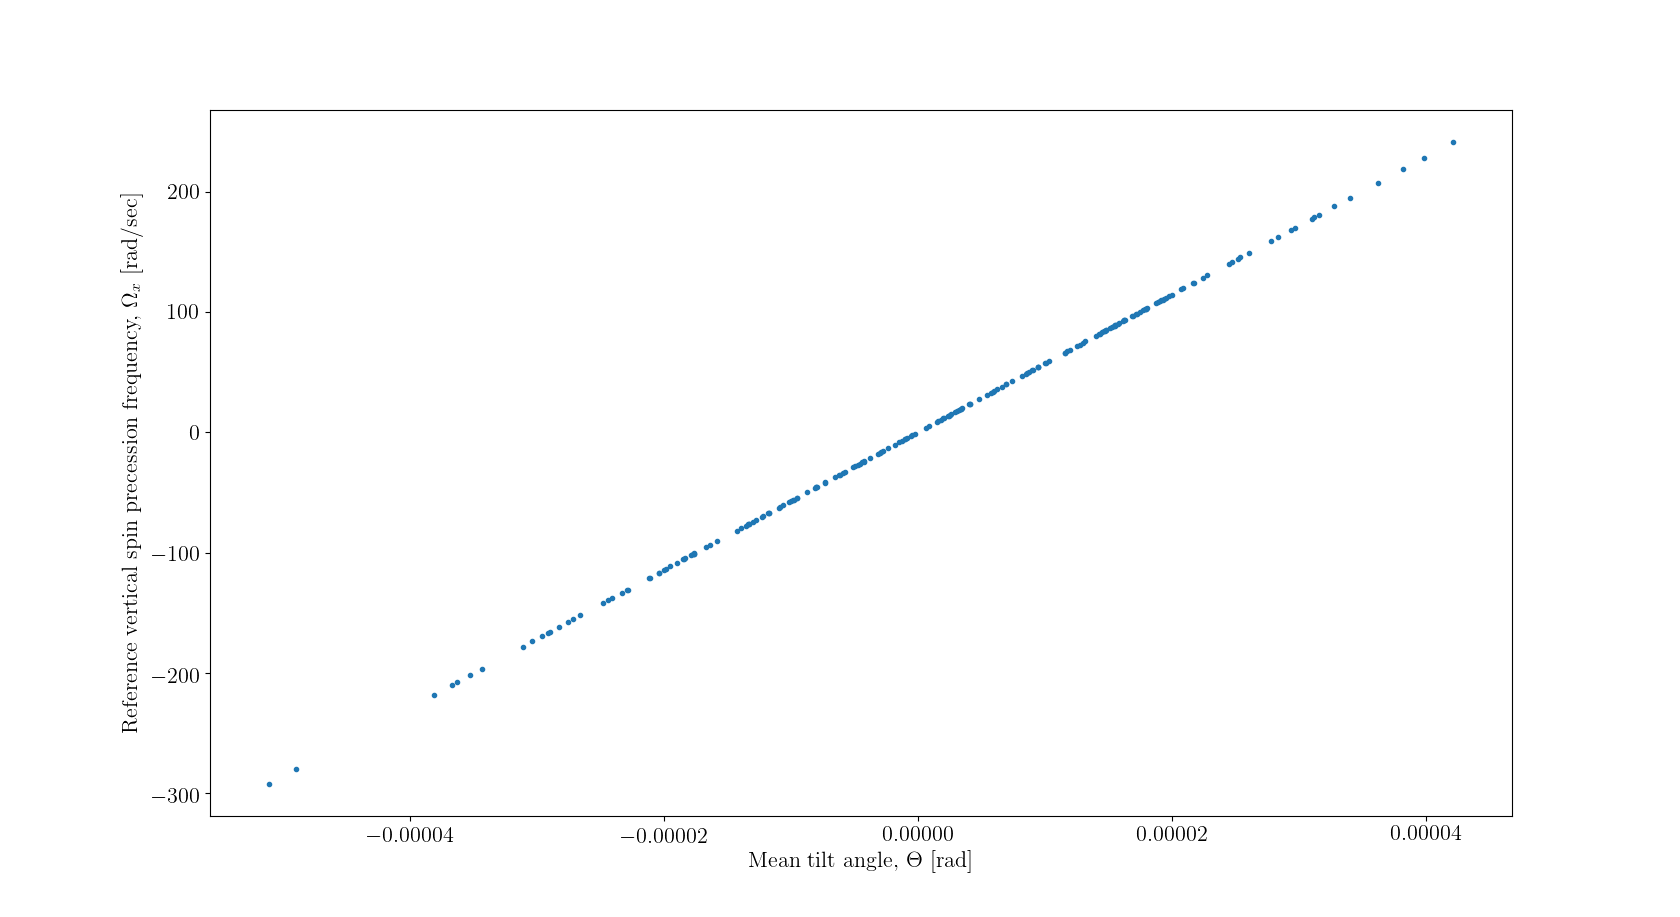
\includegraphics[scale=.45]{edm_img/Wx_dK_reference_vs_tilt_mean}}

		\subfloat[Распределение частот $\Wx$ для максимального среднего угла наклона.\label{fig:decoh_non_chi2}]{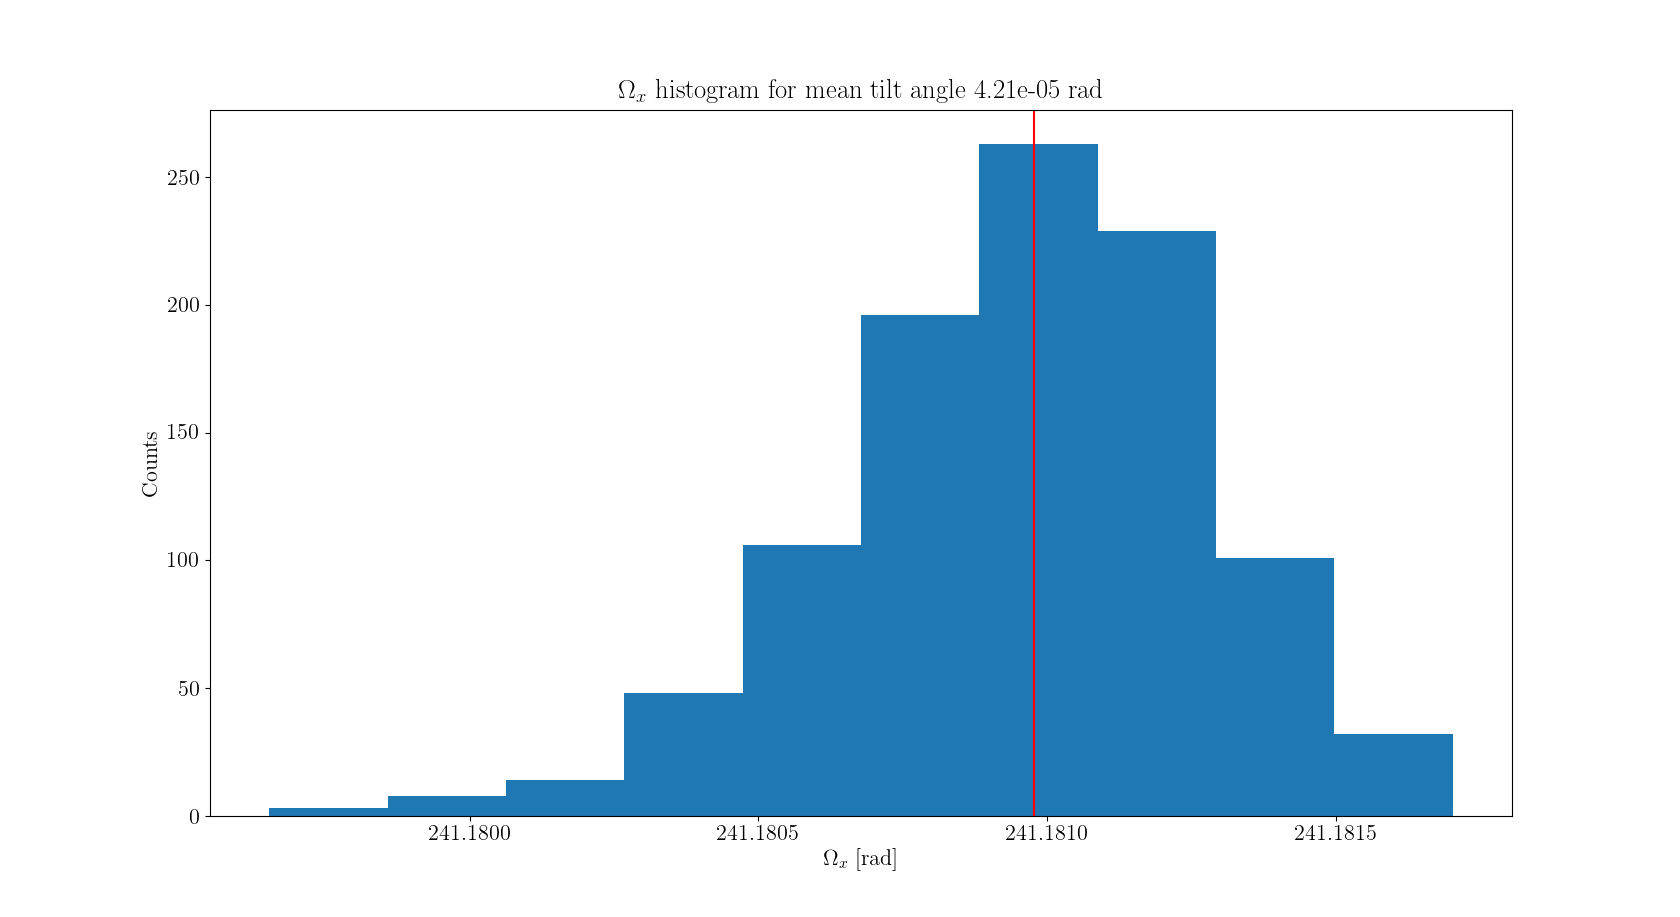
\includegraphics[scale=.45]{edm_img/Wx_dK_hist_most_positive_mean_tilt}}
	\end{figure}

	\begin{figure}[htb]\ContinuedFloat
		\centering
		\subfloat[Около-нулевое значение $\Wy$ --- результат выполнения FS условия.]{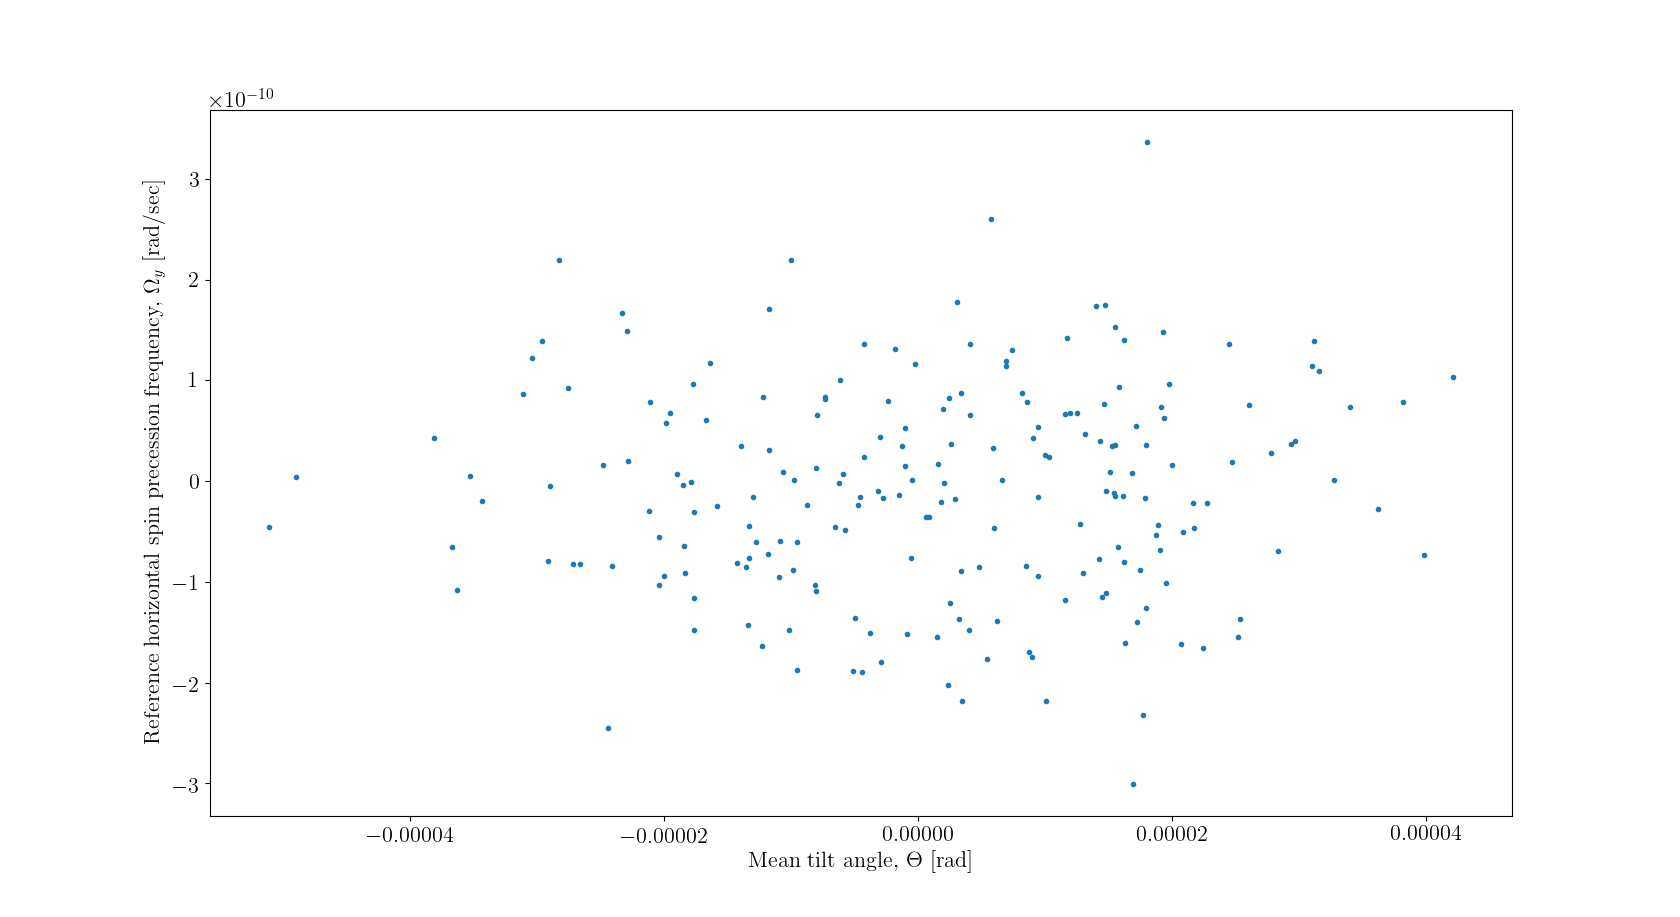
\includegraphics[scale=.45]{edm_img/Wy_dK_reference_vs_tilt_mean}}
		
		\subfloat[Распределение частот $\Wy$ для максимального среднего угла наклона.]{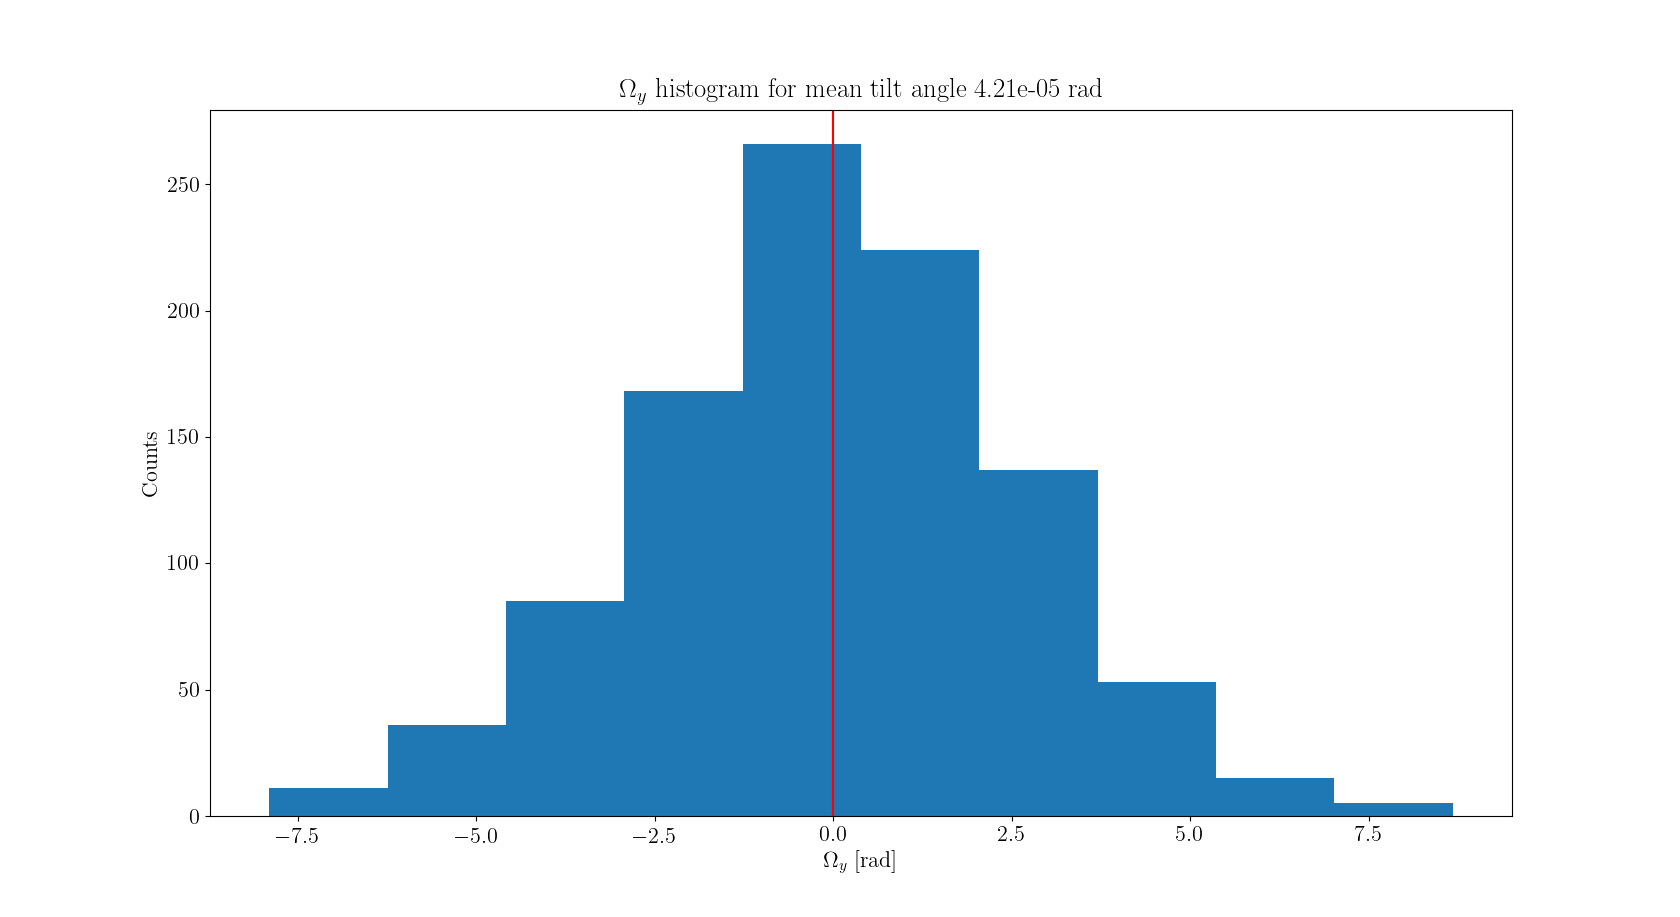
\includegraphics[scale=.45]{edm_img/Wy_dK_hist_most_positive_mean_tilt}}
		
		\caption{Моделирование декогеренции.  \label{fig:decoherence_test}}
	\end{figure}
	
	\paragraph{Сравнение декогеренции в идеальной и наклонённой FS структурах}
	Следующий тест необходим для определения влияет ли прецессия поляризации пучка в вертикальной плоскости на декогеренцию в горизонтальной. Тест был проведён следующим образом:
	\begin{itemize}
		\item Три пучка по 10 частиц: $X \sim N(0, 10^{-3}),\, Y \sim N(0, 10^{-3}), \, \Delta K \sim N(0, 10^{-4})$.
		\item Все частицы инжектированы со спином $\bld S(0) = (0, 0, 1)$.
		\item Трекинг на 1000 оборотов в идеальной и наклонённой структуре;
		\item Частоты прецессии определялись через фитирование $(turn, Sx)$  и $(turn, Sy)$.
	\end{itemize}

	Результаты моделирования представлены на рисункe~\ref{fig:cross_plot}.

	Ожидается, что зависимость частоты прецессии в горизонтальной плоскости от начального смещения частицы по $x, y, \Delta K$ от референсных значений (0, 0, 0) --- параболическая функция. Это подтверждается симуляцией для $x, y$, но не для $\Delta K$. Причиной тому является недостаточное количество синхротронных колебаний за 1000 оборотов (28), в связи с чем не происходит подавление декогеренции пучка засчёт синхротронных колебаний, отмеченное в последнем абзаце раздела~\ref{sec:BNL_Proposal}.
	
	В использованной модели кольца, отношение частоты синхротронных колебаний к частоте оборота пучка $\Omega_s/\Omega_{rev} \approx 1/35$. По этой причине, для того, чтобы ВЧ-усреднение пучка имело место, необходимое число оборотов порядка 20,000. (Это видно из рисунка~\ref{fig:mean_dK_test}) Очевидно, интегрирование не применимо в таких условиях.
	\begin{figure}[htb]
		\centering
		\subfloat[Начальное смещение по $x$]{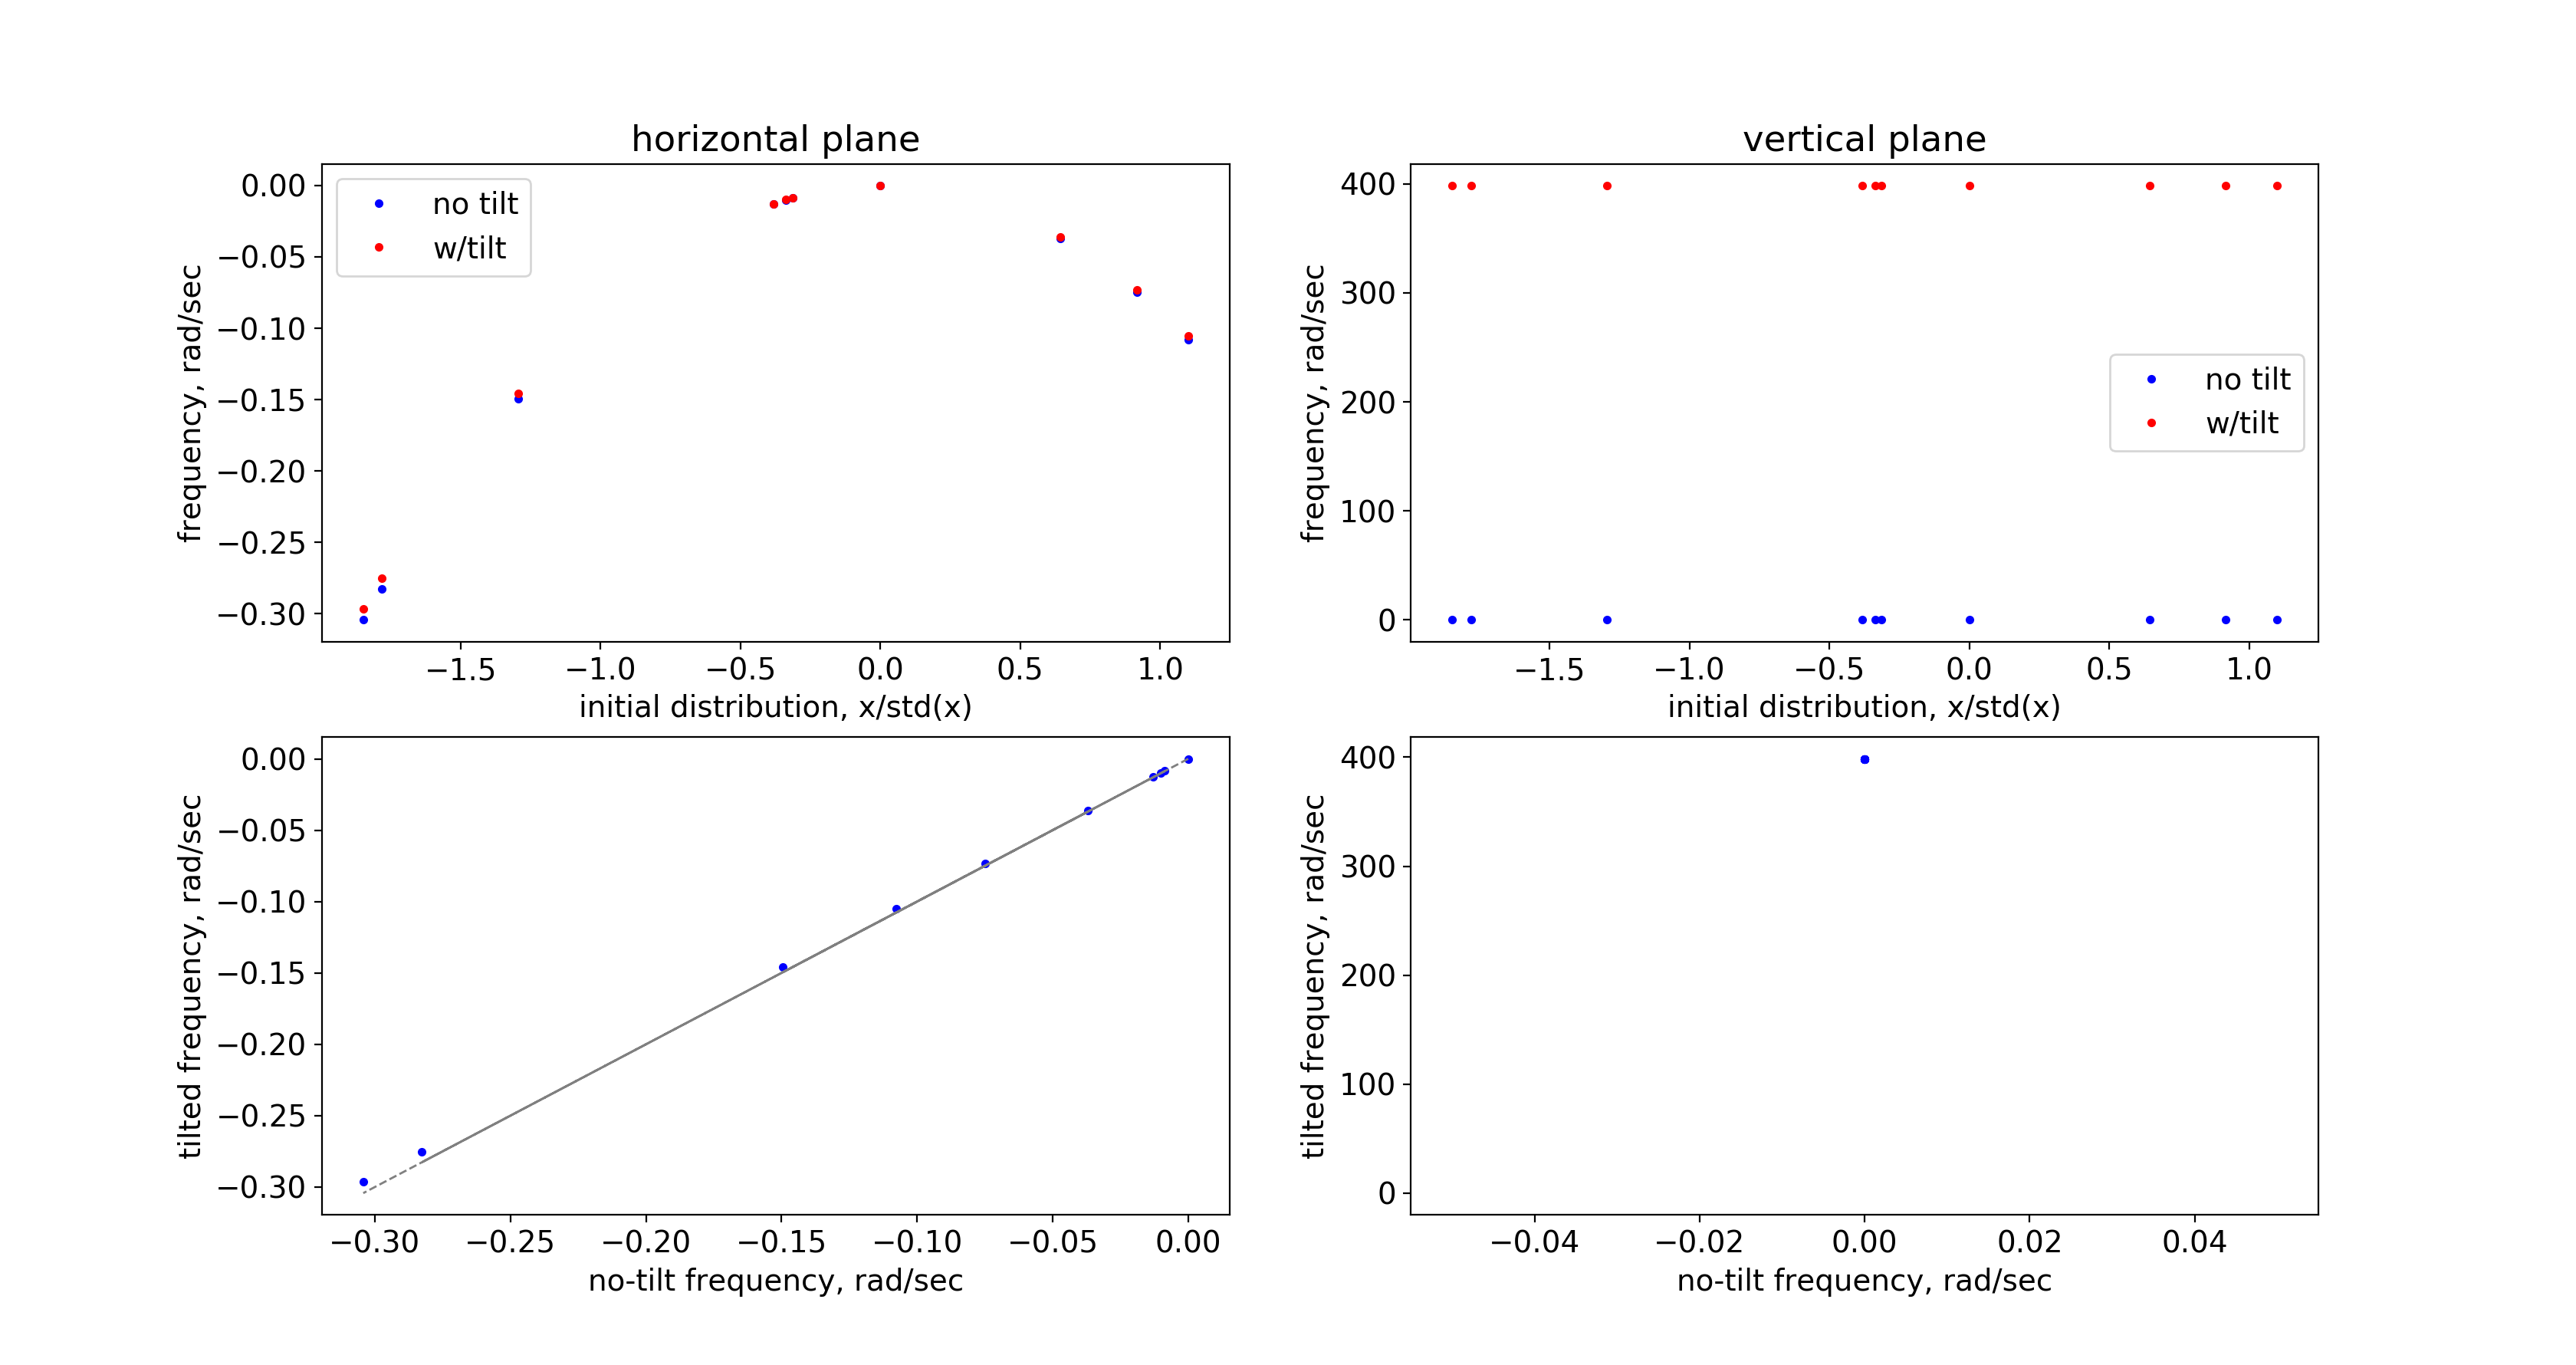
\includegraphics[scale=.45]{edm_img/cross_plot_x}}
		
		\subfloat[Начальное смещение по $y$]{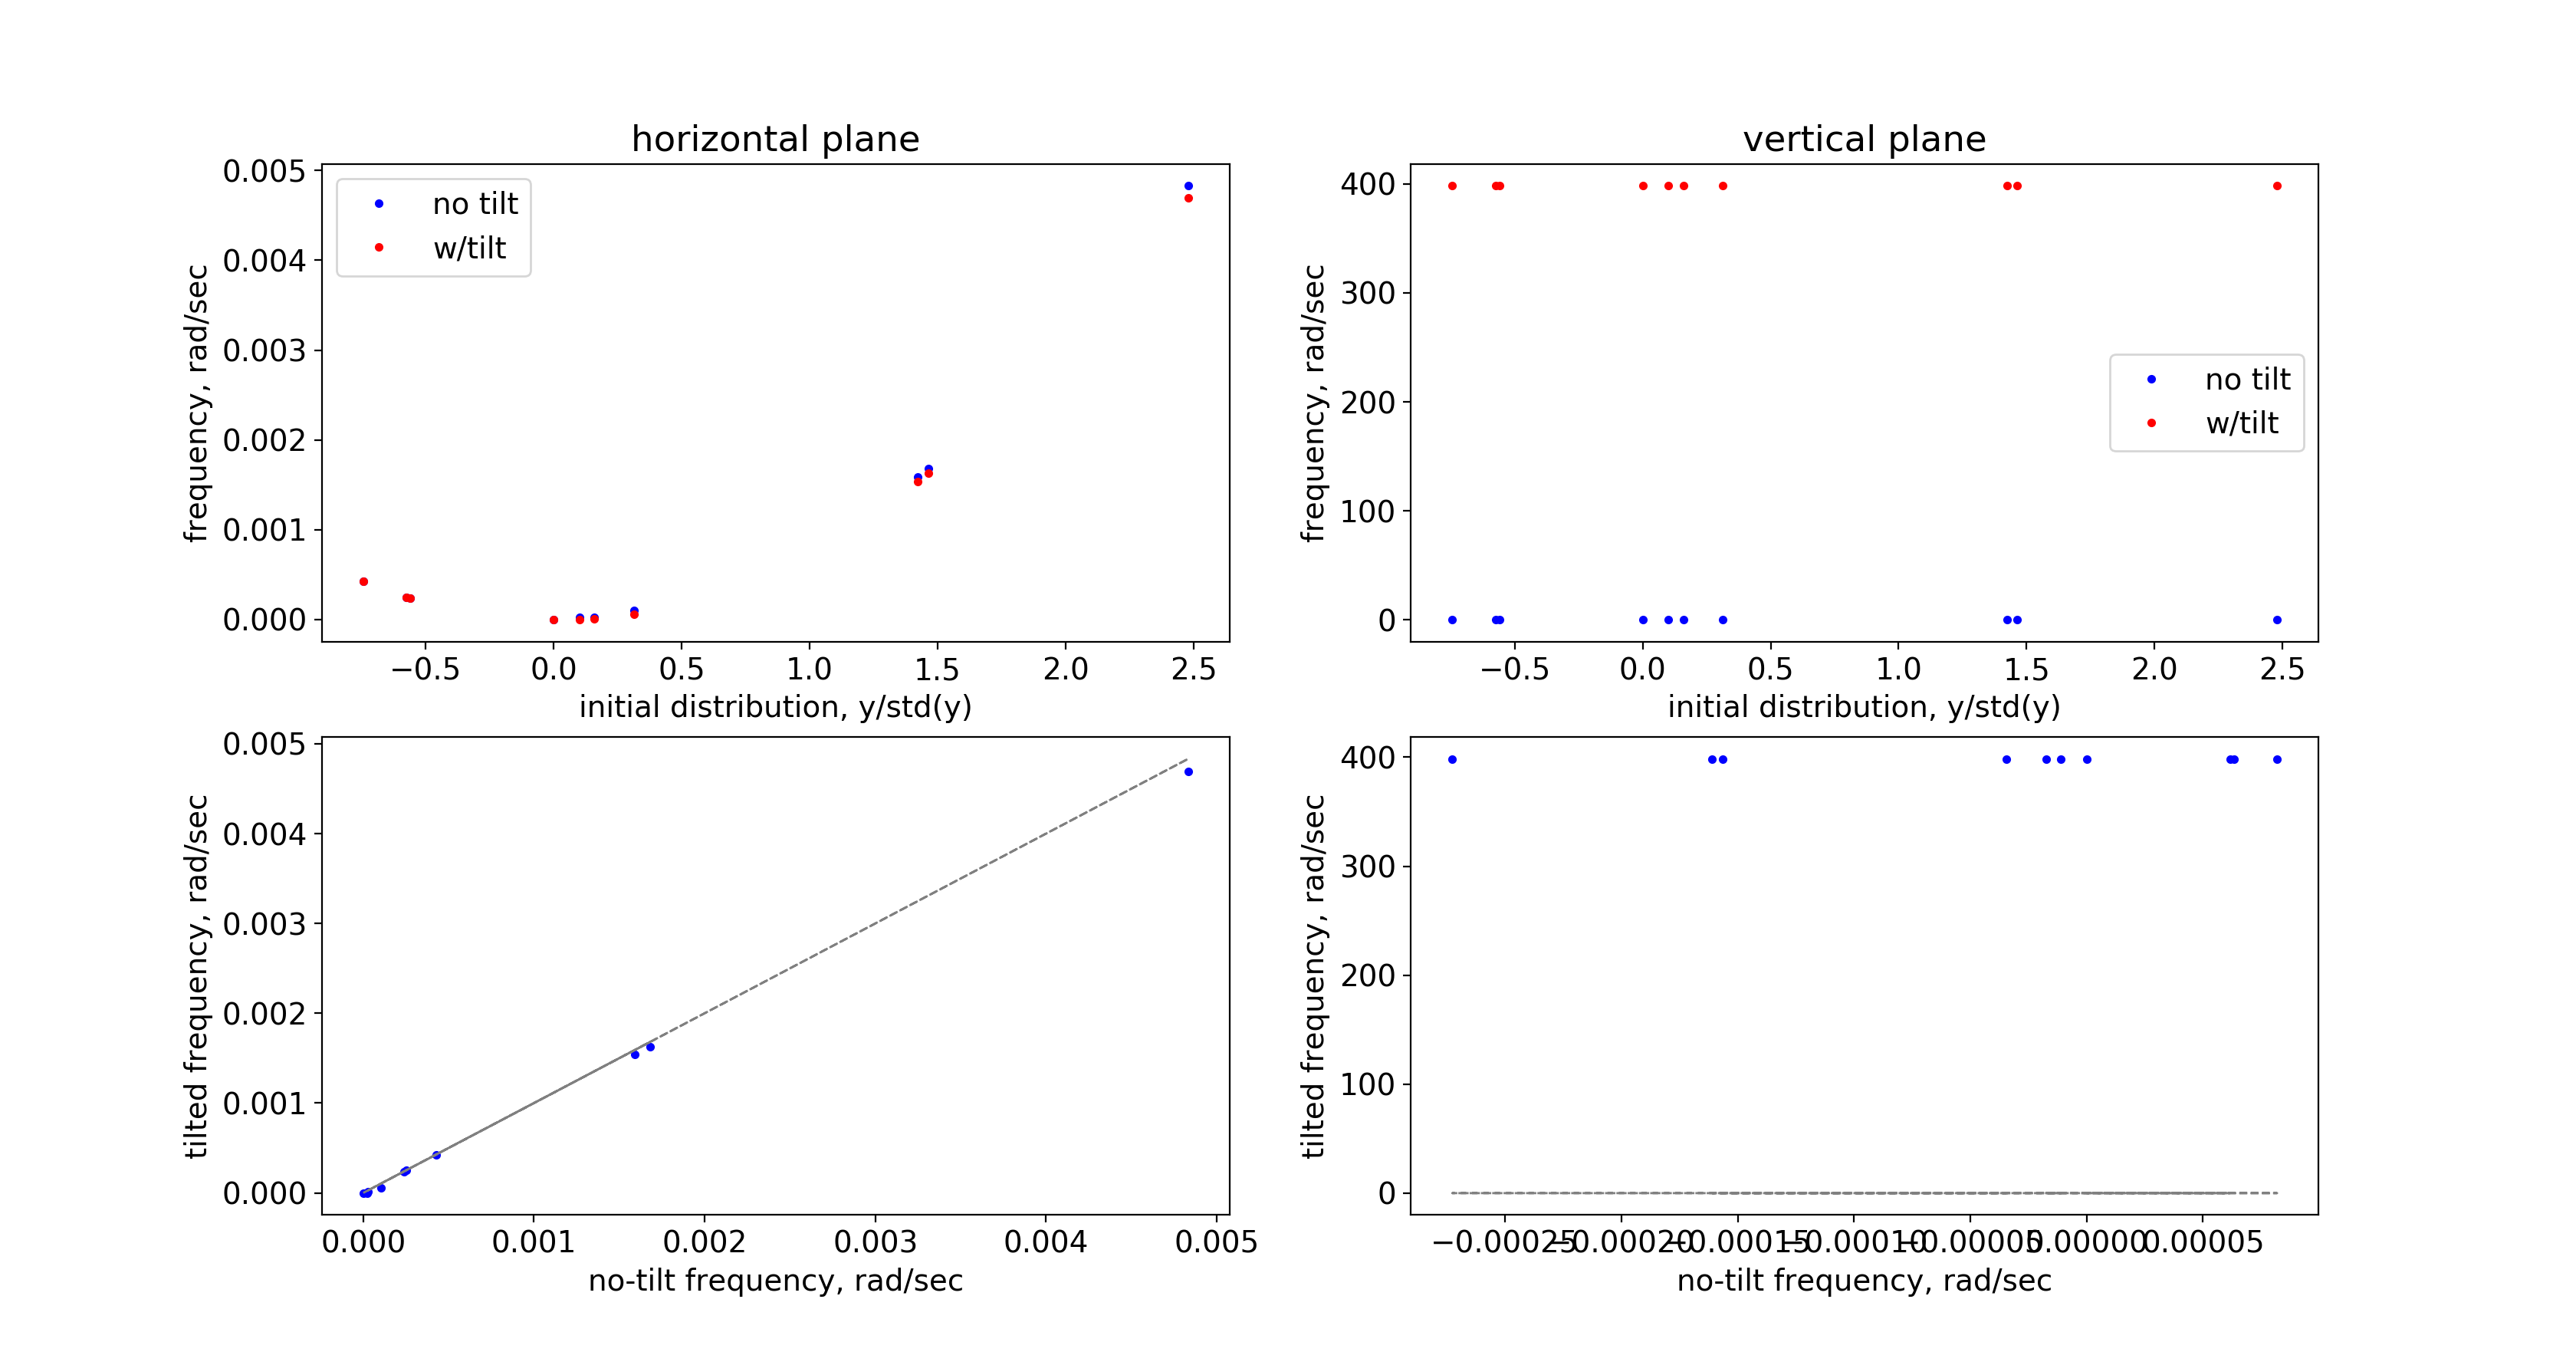
\includegraphics[scale=.45]{edm_img/cross_plot_y}}
	\end{figure}
	\begin{figure}[htb]\ContinuedFloat
		\subfloat[Начальное смещение по  $dK$]{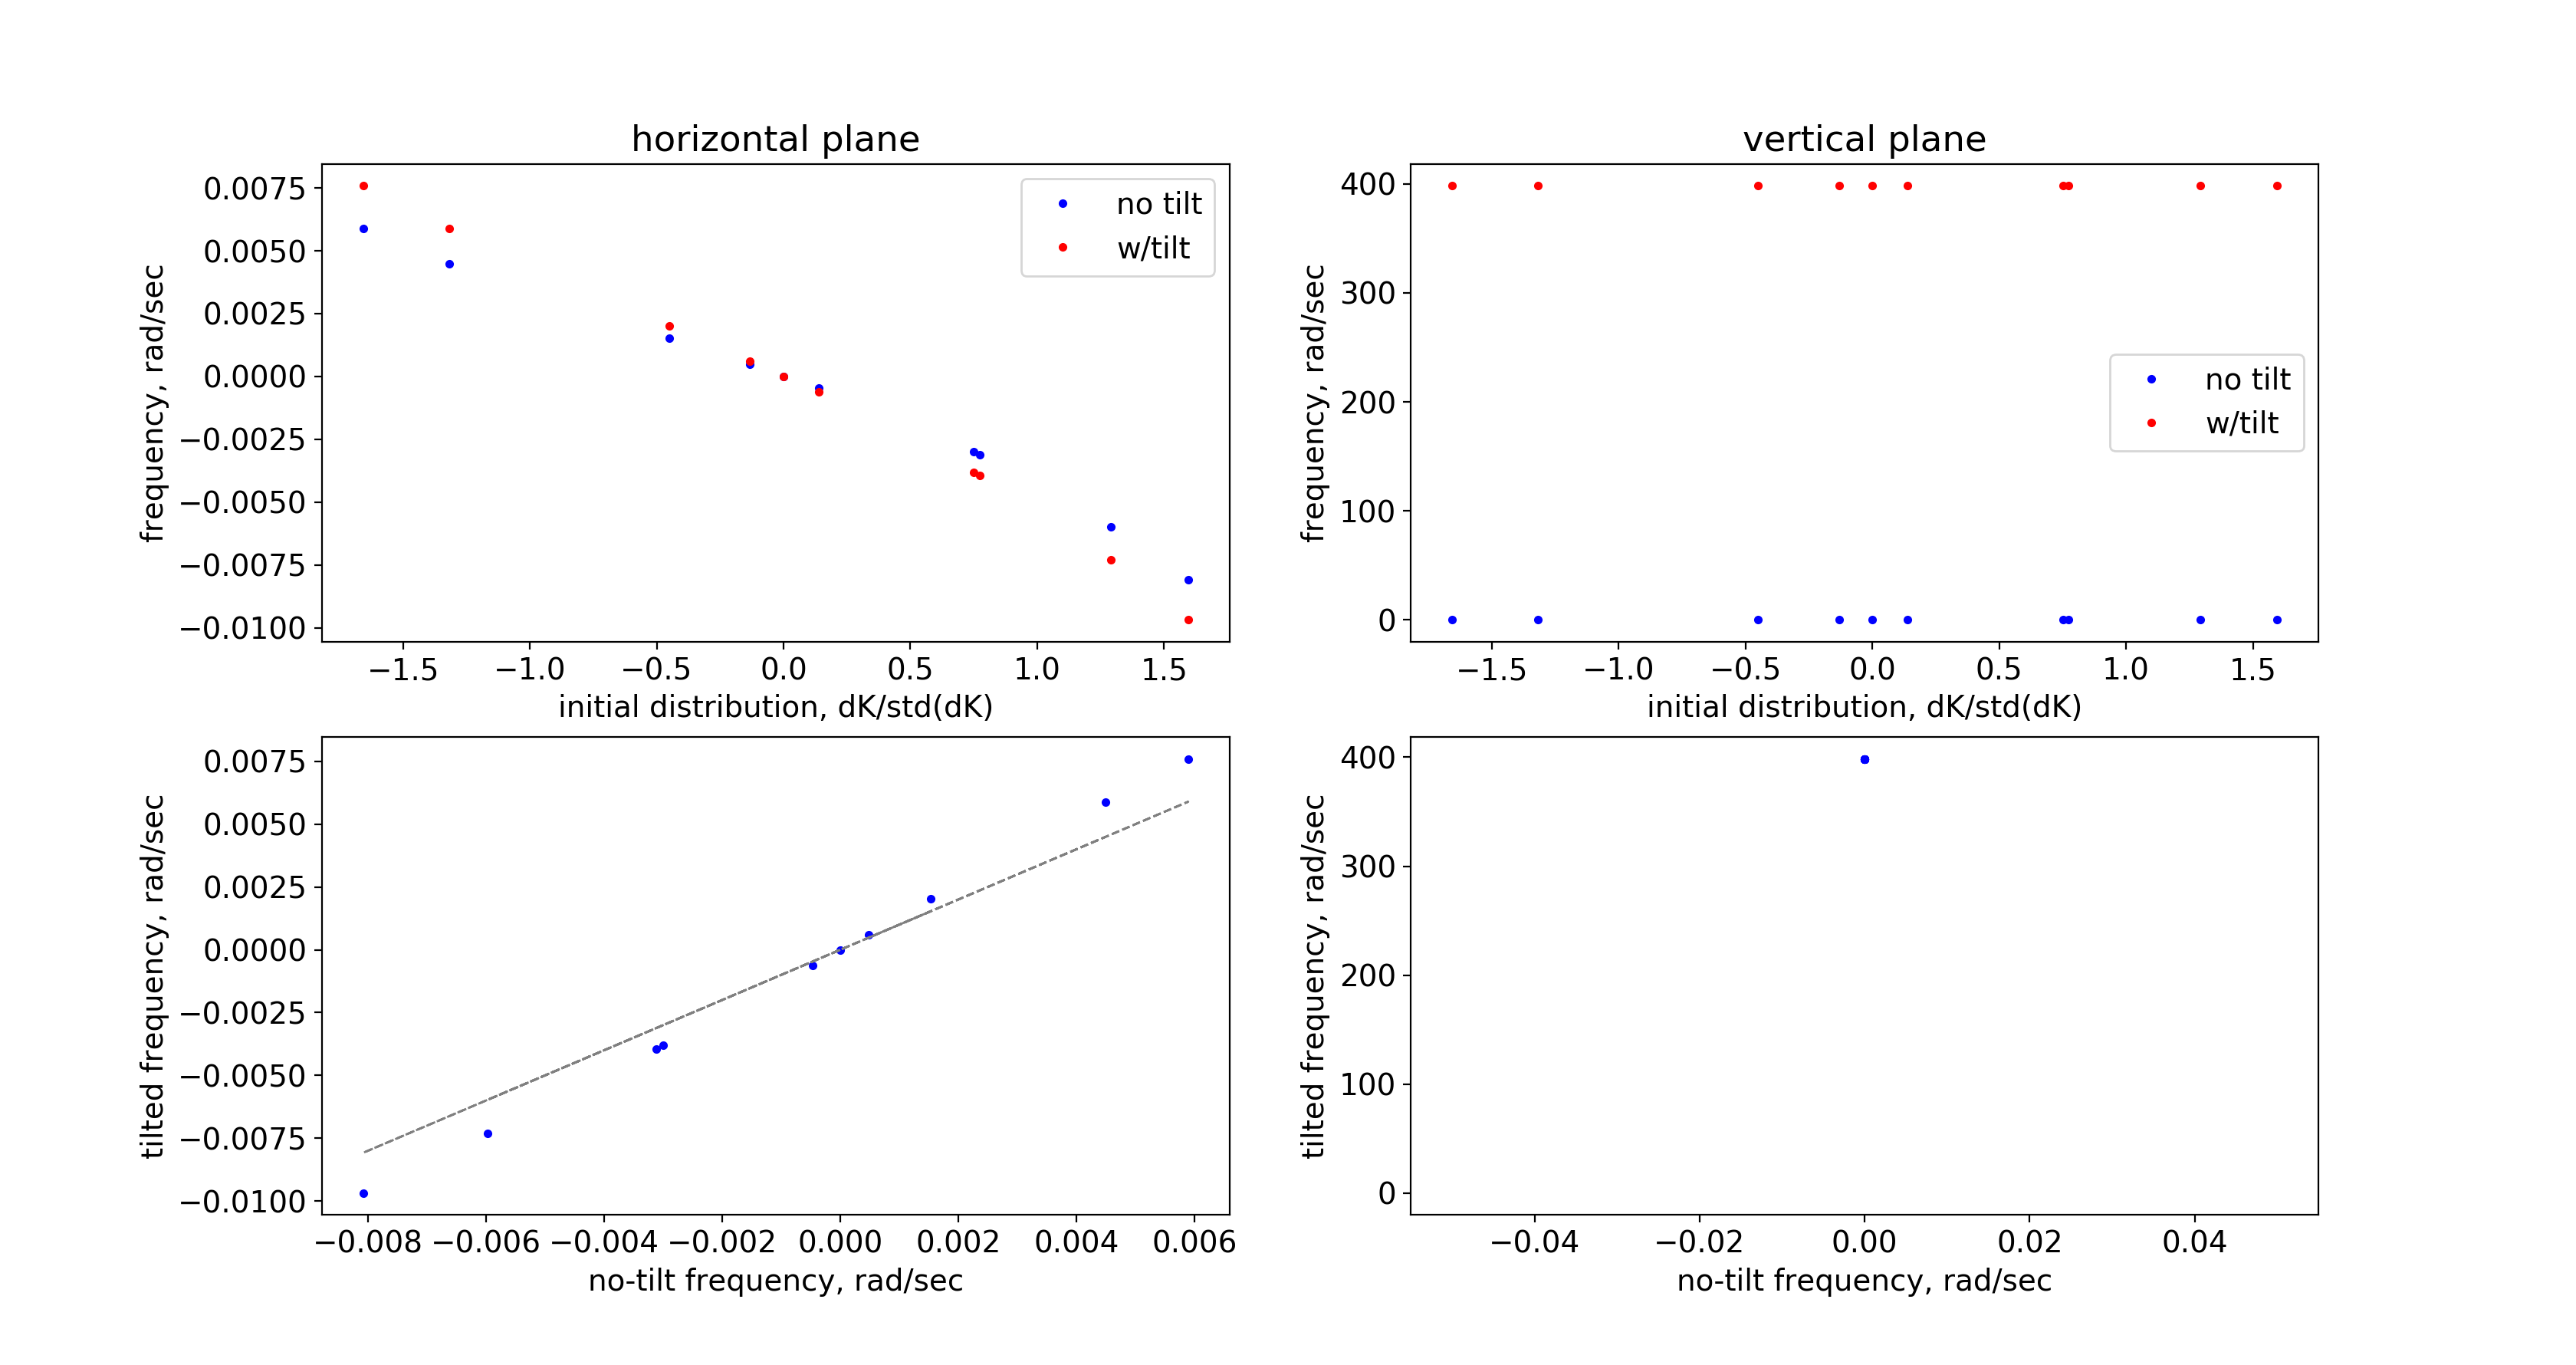
\includegraphics[scale=.45]{edm_img/cross_plot_dK}}
		\caption{Частота прецессии спина частицы в горизонтальной и вертикальной плоскости. Синий: в идеальной структуре. Красный: в структуре, со случайно наклонёнными E+B элементами. Элементы наклонены вокруг оптической оси на случайный угол из нормального распределения с нулевым средним и стандартным отклонением $10^{-4}$ радиан.\label{fig:cross_plot}}
	\end{figure}

	\begin{figure}[htb]
		\centering
		\subfloat[через 500 оборотов, $\sim$14 синхротронных колебаний. Этого недостаточно для усреднения спин-тюна в ноль, и поэтому мы не наблюдаем параболической зависимости $\avg{\Delta K} \sim \Delta K_0^{2}$.]{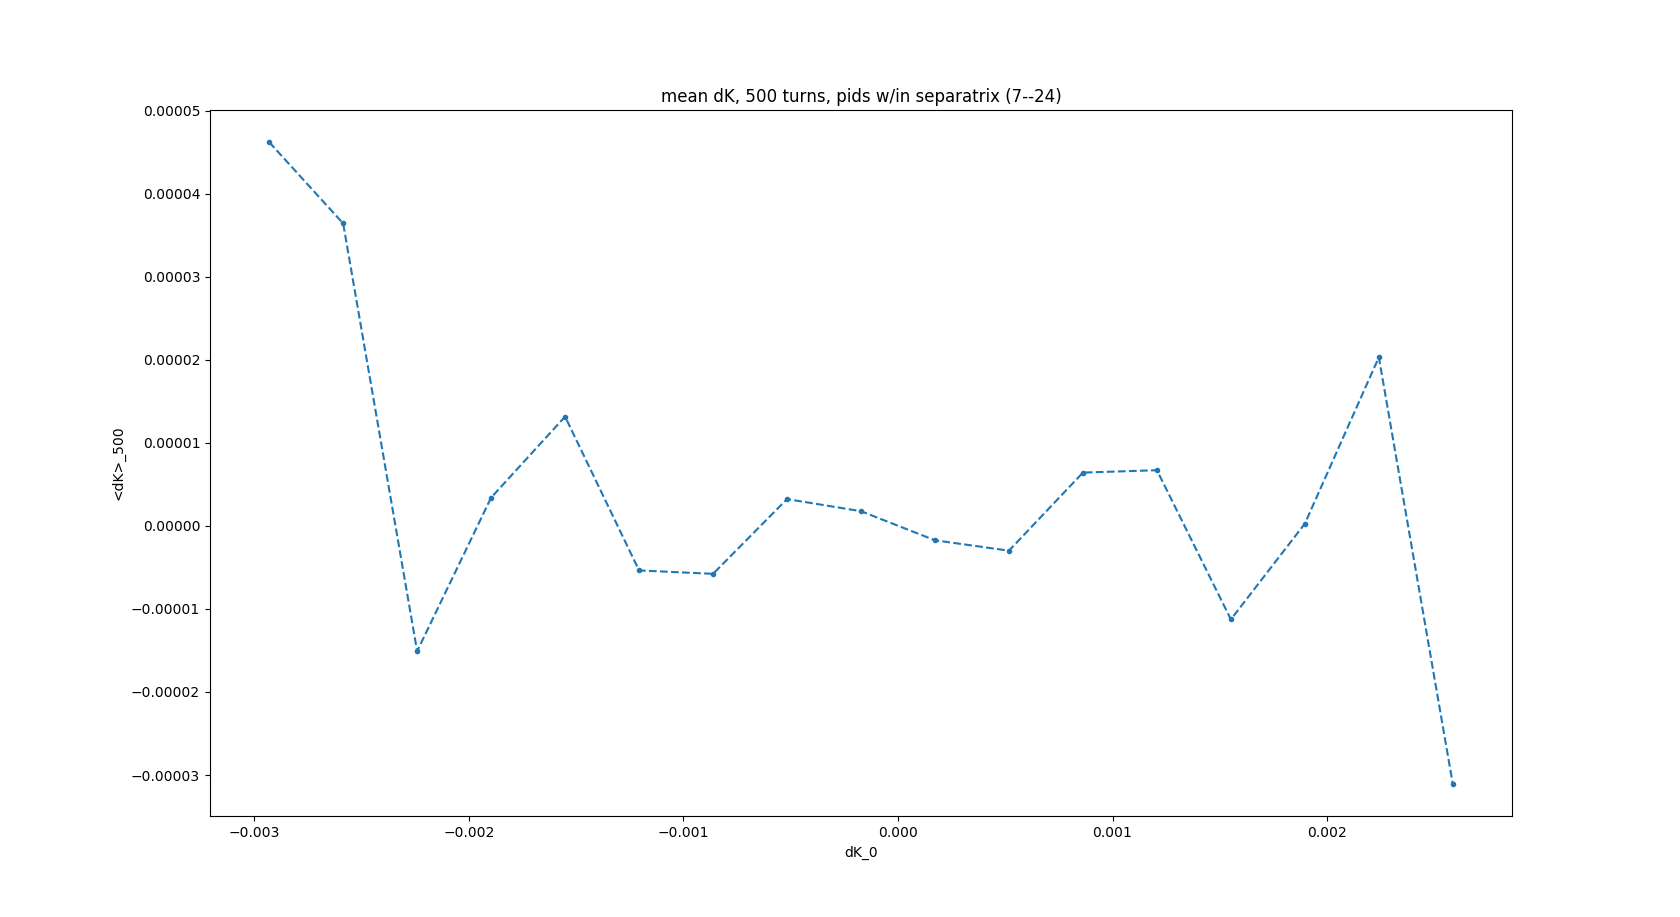
\includegraphics[scale=.4]{edm_img/mean_dK_vs_dK0_500trn}}
		
		\subfloat[через 20,000 оборотов, $\sim$571 синхротронное колебание. При таком количестве синхротронных колебаний наблюдается действие центральной предельной теоремы, происходит усреднение спин-тюна в ноль, и наблюдается параболическая зависимость $\avg{\Delta K} \sim \Delta K_0^{2}$]{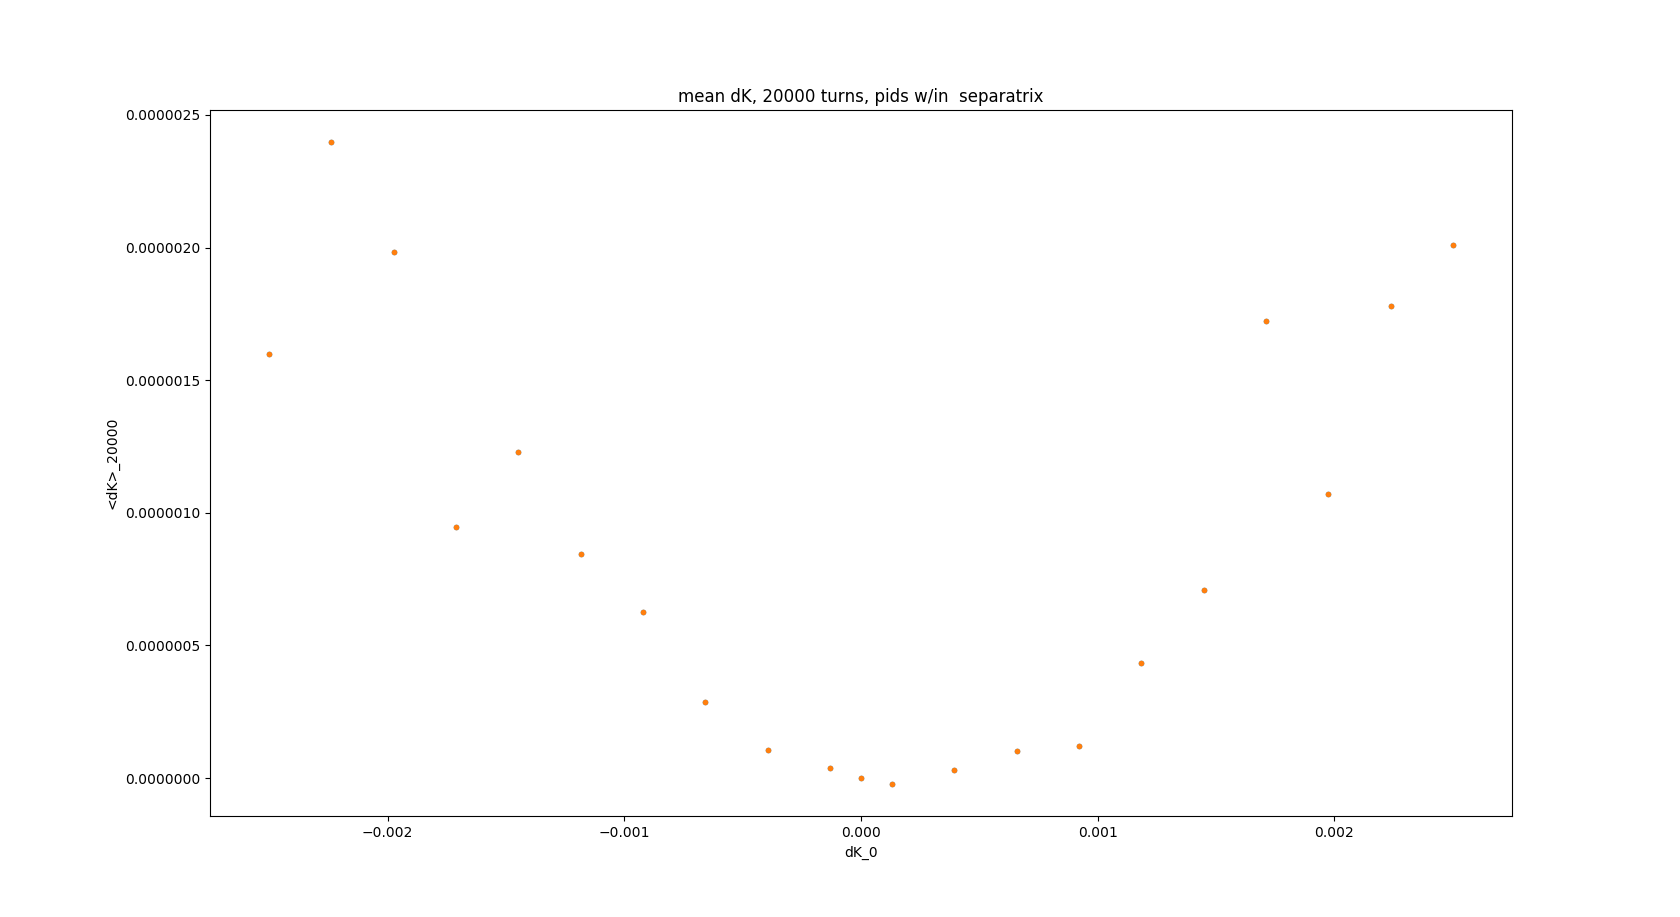
\includegraphics[scale=.4]{edm_img/mean_dK_vs_dK0_20000trn}}
		\caption{Сдвиг среднего $\avg{\Delta K}$ от референсного значения в зависимости от начального отклонения\label{fig:mean_dK_test}}
	\end{figure}
	
	\subsection{Маппинговый код}
	
	По этой причине на данный момент разрабатывается маппинговый код. 
	
	\clearpage
	\begin{thebibliography}{99}
		\bibitem{Pretz_presentation}
		Pretz J 2012 Measurement of Permanent Electric Dipole Moments of Proton, Deuteron, and Light Nuclei in Storage Rings. Презентация. \url{http://collaborations.fz-juelich.de/ikp/jedi/public_files/usual_event/2012-06-18_J.Pretz_SSP2012.pdf}
		
		\bibitem{BNL}
		Anastassopoulos D et al. 2008 AGS Proposal: Search for a permanent electric dipole moment of the deuteron nucleus at the $10^{-29}$ e$\cdot$cm level. Отчёт BNL. \url{https://www.bnl.gov/edm/files/pdf/deuteron_proposal_080423_final.pdf}
		
		\bibitem{Proton_EDM}
		Anastassopoulos D et al. 2015 A Storage Ring Experiment to Detect a Proton Electric Dipole Moment. \url{http://arxiv.org/abs/1502.04317}
		
		\bibitem{SenichevRuPAC2016}
		Senichev Y 2016 Search for the Charged Particle Electric Dipole Moments in Storage Rings. Proc. RuPAC2016 (St. Petersburg, Russia).

		\bibitem{SenichevICAP15}
		Senichev Y 2015 Investigation of lattice for deuteron EDM ring. Proc. ICAP2015 (Shanghai, China).
		
		\bibitem{Ivanov_thesis}
		Иванов А Нелинейное матричное интегрирование спин-орбитальной динамики заряженных частиц. СПбГУ; 2015.
	\end{thebibliography}
\end{document}